\section*{Введение}
\addcontentsline{toc}{section}{Введение}

Производственную практику я проходила в компании Surf (ООО “СёрфСтудио”).

Surf – одна из ведущих студий мобильной разработки и дизайна в России, обладающая богатым опытом работы с крупными сервисами. Студия специализируется на электронной коммерции и мобильном банкинге, а процессы создания продуктов тесно связаны с пониманием задач бренда. Ключевые направления работы включают создание качественных приложений с привлекательным дизайном, а также их всестороннюю поддержку. Это предполагает активное взаимодействие с клиентами на стадии разработки и полноценное сопровождение продукта после его выпуска.

Компания зарекомендовала себя как на российском рынке, так и за рубежом. Среди её крупных клиентов такие компании, как Medium Quality, Forbes, Банк «Зенит», Промсвязьбанк, Триколор и Delivery Club. Surf ежегодно занимает высокие позиции в различных рейтингах мобильных разработчиков, что подтверждает высокое качество её продуктов.

Целью моей практики было овладение основами языка программирования Swift и разработка приложений под iOS. В качестве основного проекта было выбрано приложение "Персонажи сериала Рик и Морти". Приложение должно было состоять из двух экранов: список персонажей и детальная информация о конкретном персонаже, с использованием данных из открытого API.

\textbf{Требования к приложению "Персонажи сериала Рик и Морти":}

\textbf{Экран со списком персонажей:}
\begin{itemize}
    \item Экран состоит из вертикального списка ячеек с информацией о персонажах,
    \item Список можно скроллить,
    \item В ячейке отображаются имя (не больше 1 строки), статус, раса/вид, пол и изображение персонажа,
    \item При нажатии на ячейку можно перейти к экрану детальной информации,
    \item Отображаются персонажи первой страницы запроса /character (20 штук).
\end{itemize}

\textbf{Экран детальной информации о персонаже:}
\begin{itemize}
    \item На экране отображаются изображение, имя, статус, раса/вид, пол, список эпизодов, в которых появляется персонаж, и последнее известное местоположение,
    \item Список эпизодов отображается в формате “1, 4, 13”, где числа – это id эпизодов из массива "episode".
\end{itemize}

Помимо работы с Swift, я также изучала язык Dart и фреймворк Flutter для создания мобильных приложений. В рамках этой части практики мне было дано задание создать приложение-галерею фотографий, которое должно было включать три страницы: главную страницу с сеткой фотографий, страницу карусели фотографий и страницу ошибки. Помимо этого, приложение должно было поддерживать светлую и тёмную темы, а также загрузку фотографий из галереи пользователя в облачное хранилище.

\begin{figure}[h]
    \centering
    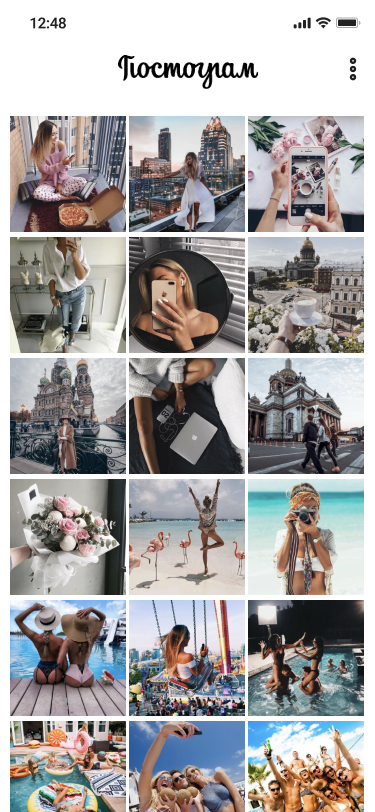
\includegraphics[width=0.2\linewidth]{images/postogram.png}
    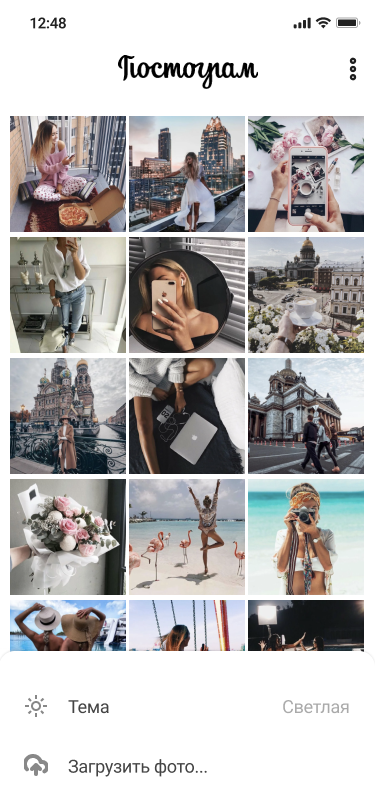
\includegraphics[width=0.2\linewidth]{images/postogrammenu.png}
    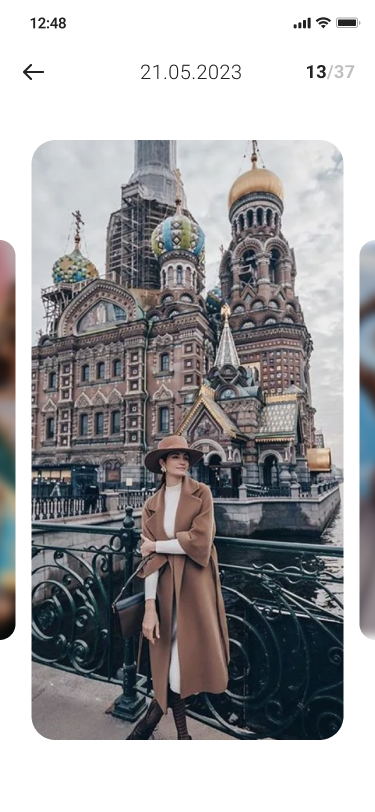
\includegraphics[width=0.2\linewidth]{images/photo.png}
    
\includegraphics[width=0.2\linewidth]{images/postogramerror.png}
    \caption{Приложение-галерея фотографий}
\end{figure}

\textbf{Техническое задание:}

\begin{enumerate}
    \item Приложение включает три страницы: главную страницу с сеткой фотографий, страницу карусели фотографий и страницу ошибки.
    \item На главной странице в навигационной панели должно быть название приложения ("Постограмм") и справа от него кнопка. При нажатии на кнопку должно появляться окно с выбором темы (светлой и тёмной) и загрузки фотографий из галереи.
    \item При нажатии на любую из фотографий в сетке открывается карусель изображений для выбранной фотографии. В заголовке отображается дата создания фотографии, справа от него указан номер текущей фотографии и общее количество фотографий. Слева от заголовка есть кнопка для возврата на главную страницу.
    \item При возникновении ошибки в работе приложения пользователю отображается страница ошибки с заголовком ошибки и кнопкой "назад".
    \item Приложение анимируется по усмотрению разработчика.
    \item Приложение подключено к облачному хранилищу и отображает все доступные фотографии из него.
    \item При нажатии на кнопку "Загрузить фото" приложение открывает файлы на устройстве пользователя, загружает их в облачное хранилище и отображает в галерее.
\end{enumerate}


